\documentclass[twocolumn, 9pt]{jsproceedings}
\RequirePackage[l2tabu, orthodox]{nag}  % 古いコマンドやパッケージを使用した場合に警告する
\usepackage[all, warning]{onlyamsmath}  % amsmath が提供しない数式環境を使用した場合に警告する
% \usepackage{flushend}  % 最終ページの2カラムの左右の高さを揃える



\usepackage{otf}
\usepackage[ipa]{pxchfon}
\usepackage{caption}
\usepackage{graphicx}

% タイトル
\title{つくばチャレンジ 2023 における\\千葉工業大学未来ロボティクス学科 box2,box3チームの取り組み}

\author{○今井 悠月,井口 颯人,樋高 聖人,春山 健太,藤原 柾,\CID{8705}橋 祐樹,白須 和暉,野村 駿斗,
望月 悠矢,\\馬場 琉生,村林 孝太郎,桜井 真希,中村 雄一,長島 昂生,\\上田 隆一,林原 靖男(千葉工大)}

\etitle{The activities of the Advanced Robotics Department box2 and box3 team of Chiba Institute of Technology in the Tsukuba Challenge 2023}

\eauthor{Yuzuki IMAI, Hayato IGUCHI, Masato HIDAKA, Kenta HARUYAMA, Masaki FUJIWARA, \\Yuki TAKAHASHI,
 Kazuki SHIRASU, Hayato NOMURA, Yuya MOCHIZUKI, Ryusei BABA, \\Koutarou MURABAYASHI, Maki SAKURAI,
 Yuichi NAKAMURA, Kousei NAGASHIMA, \\Ryuichi UEDA and Yasuo HAYASHIBARA (CIT)}

\affiliation{千葉工業大学未来ロボティクス学科 box2, box3チーム}

\abstract{
  In this paper, we present the activities of the Advanced Robotics Department box2 and box3 team of 
  Chiba Institute of Technology in the Tsukuba Challenge 2023. 
  We developed autonomous outdoor mobile robots, and we tackled several challenges. 
  For example, We developed robots using machine learning and robots that can run in the rain.
}


\begin{document}
\maketitle

% 本文
\section{緒言}
我々は,屋外でも正確に自律移動可能なロボットを目指し,その研究および開発の一環として
つくばチャレンジに参加している.
これまで本研究室\footnote{千葉工業大学未来ロボティクス学科 林原研究室}では,地図生成や自己位置推定を
中心に研究開発を行ってきた.近年では,防水機能や高い拡張性を有したオープンプラットフォームのロボットの
開発も行っている.
つくばチャレンジ2022では,開発したロボットやシステムを用いて,記録走行において完走を達成した.
しかし,今年度からは確認走行エリアのコースが一部変更され,つくば市役所の外周がコースに含まれるようになった.
そのため,30 m 程度の 2次元レーザレンジセンサ 1つでは,低層の茂みや障害物などを検出しつつ,
安定して自己位置推定を行うのが困難となった.
また,道幅の狭い経路を通る必要があるため,従来のシステムよりもロバストなシステムが要求された.
本稿では,このような問題を解決するためにつくばチャレンジ2023に向けて取り組んだ内容に関して紹介する.

\section{開発中のロボット}
ロボットを常に屋外環境で走行させるためには,防水設計が求められる.ただし,防水性を担保しながら
ロボットの機構や電気回路の追加および変更を行うことは,作業の負担が大きいと考えられる.
さらに,これらの作業には多くの時間を要するため,新たなアルゴリズムの開発や検証に十分な時間を割当てられない
ことが問題となっていた.

このような問題を踏まえ,本研究室では屋外自律移動ロボットプラットフォーム ORNE-boxの開発を行ってきた\cite{box}.
日々検証と改良を重ねており,現在は,3台のロボット(ORNE-box,ORNE-box2,ORNE-box3)がある.
これらのロボットは,屋外での自律走行を目的としており,屋外自律走行の研究開発に必要な機能をパッケージ化
し,提供することを目標に開発を行っている.現在はウェブページ上にて設計データなどを順次公開している.

ORNE-box2 は,ORNE-box の問題点を洗い出し改善を図るという方針のもと,昨年度から開発を行っている.
センサ構成などに差異はあるが,基本的なシステム構成は同じである.

ORNE-box3 は,今年度から開発を行っており,ORNE-box2 の防水性能をさらに強化したものとなっている.

\subsection{ハードウェア}
次に,ORNE-box-Series の外観を\figref{fig:orne-series},ハードウェア構成を\tableref{table:1}に示す.
これらのロボットは,i-Cart middle をベースとしている.

\begin{figure}[h]
  \centering
  \begin{minipage}[b]{0.3\linewidth}
    \centering
    \includegraphics[width=21.1mm]{fig/box.pdf}
    \caption*{(a) ORNE-box}
  \end{minipage} 
  \hspace{-1.2mm}
  \begin{minipage}[b]{0.3\linewidth}
    \centering
    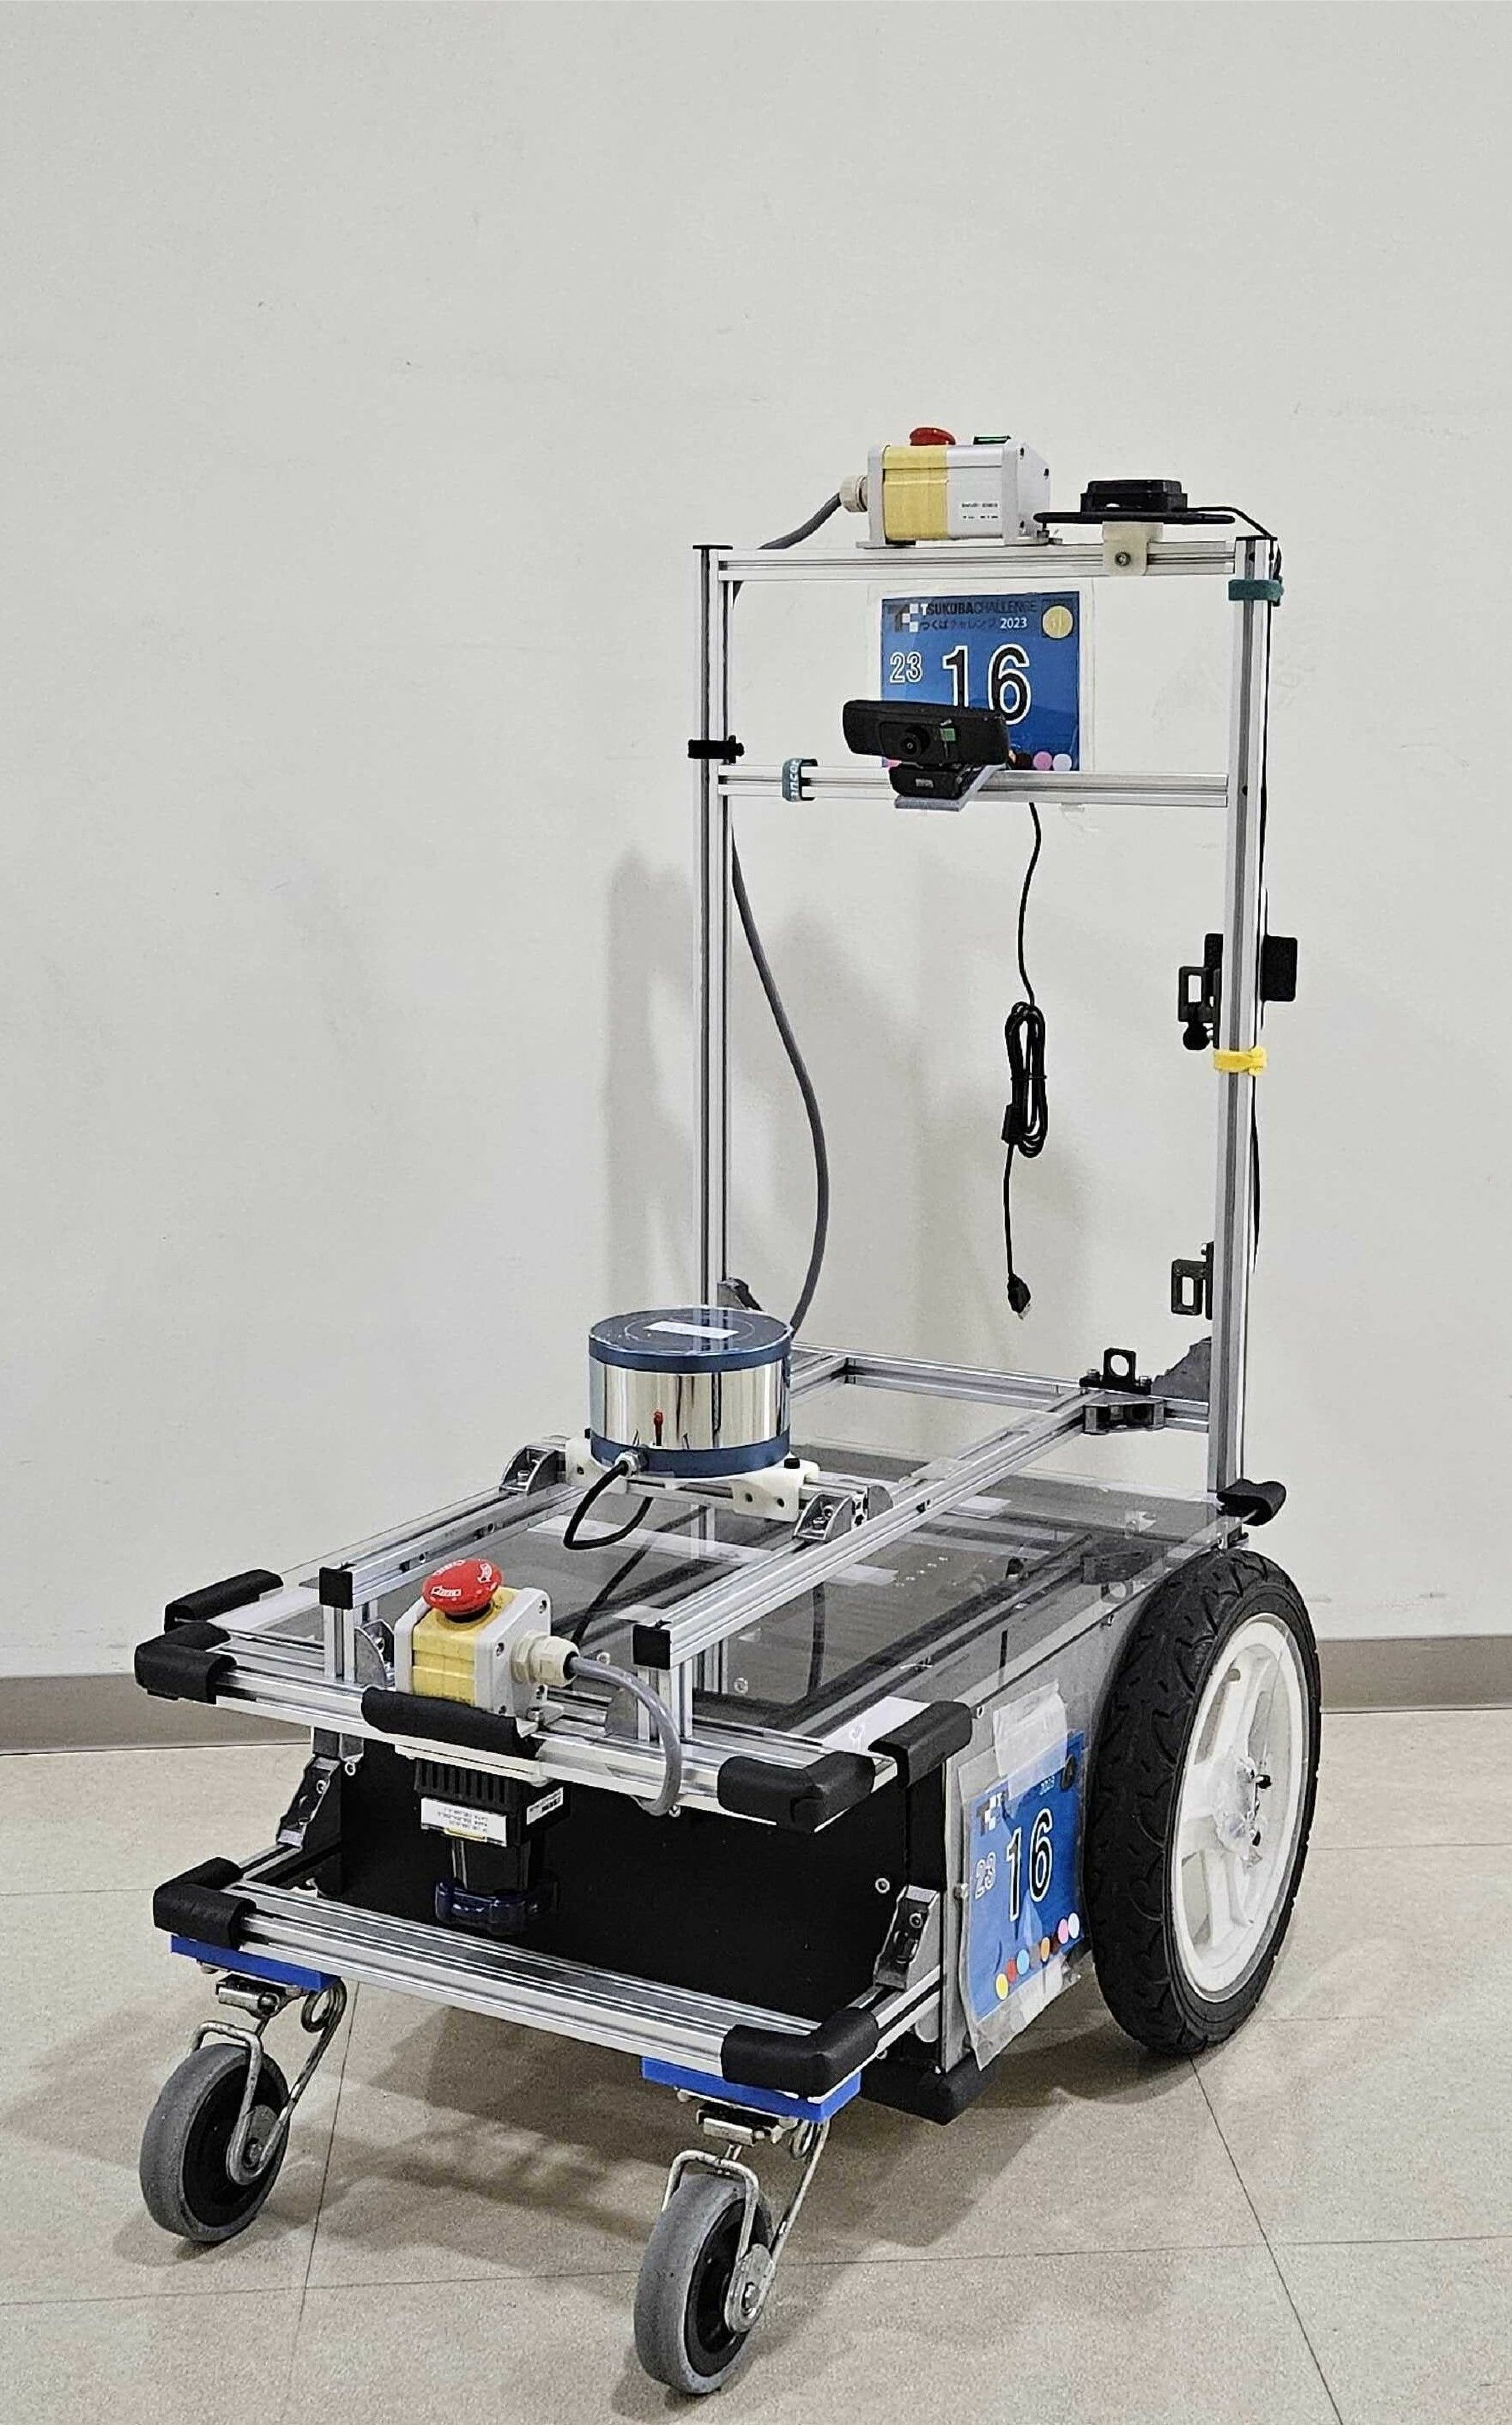
\includegraphics[height=34mm]{fig/box2.pdf}
    \caption*{(b) ORNE-box2}
  \end{minipage}
  \begin{minipage}[b]{0.3\linewidth}
    \centering
    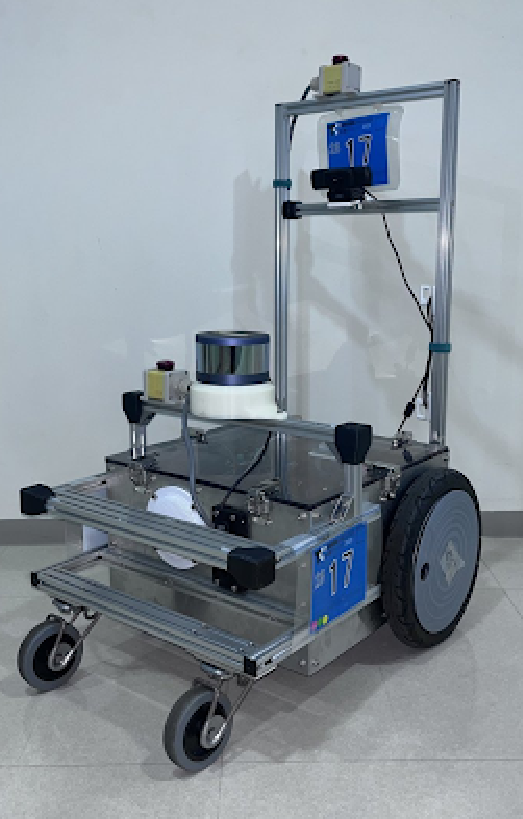
\includegraphics[height=34mm]{fig/box3.pdf}
    \caption*{(c) ORNE-box3}
  \end{minipage}
  \caption{ORNE-box-Series}
  \label{fig:orne-series}
\end{figure}


\begin{table}[h!]
  \centering
    \caption{Specifications of the robots}
    \label{table:1}
    \scalebox{0.72}{
    \begin{tabular}{|l||c|c|c|}  \hline
       & ORNE-box & ORNE-box2 & ORNE-box3 \\ \hline \hline
      Depth[mm] & \multicolumn{2}{c|}{600} & ??? \\ \hline
      Wide[mm] & \multicolumn{2}{c|}{506.5} & ??? \\ \hline
      Height[mm] & \multicolumn{2}{c|}{957} & ??? \\ \hline
      Wheel diameter[mm] & \multicolumn{3}{c|}{304}\\ \hline
      Battery & \multicolumn{3}{c|}{LONG WP14-12SE}\\ \hline
      Motor & \multicolumn{3}{c|}{Oriental motor TF-M30-24-3500-G15L/R}\\ \hline
      Driving system & \multicolumn{3}{c|}{Power wheeled steering}\\ \hline
      2D-LiDAR & URM-40LC-EW & None & UTM-30LX-EW\\
      & (HOKUYO) & & (HOKUYO)\\ \hline
      3D-LiDAR & None & \multicolumn{2}{c|}{R-fans-16} \\
      & & \multicolumn{2}{c|}{(SureStar)}\\ \hline
      IMU & ADIS16465 & ADIS16470 & None\\ 
      & (Analog devices) & (Analog devices) & \\ \hline
      Camera & None & \multicolumn{2}{c|}{CMS-V43BK}\\ 
      &  & \multicolumn{2}{c|}{(Sanwa supply)}\\ \hline
    \end{tabular}
  }
  \end{table}


\subsection{ソフトウェア}
本研究室では,従来より ROS(Robot Operating System)のnavigation stack\cite{navigation}を基に開発された
システムであるorne\_navigation\cite{orne-navigation} と orne\_box\cite{orne-box} により,ロボットを自律走行させている.
\figref{fig:soft-fig}に開発しているロボットのソフトウェアを含むシステム構成を示す.
このシステムは,LiDARとオドメトリを用いた Monte Carlo Localization(MCL)により確率的に自己位置を推定し, 
経路計画に基づいて自律走行している.なお,両ソフトウェアは GitHubのopen-rdc\cite{open-rdc} で公開している.\\

\begin{figure}[h!]
  \centering
  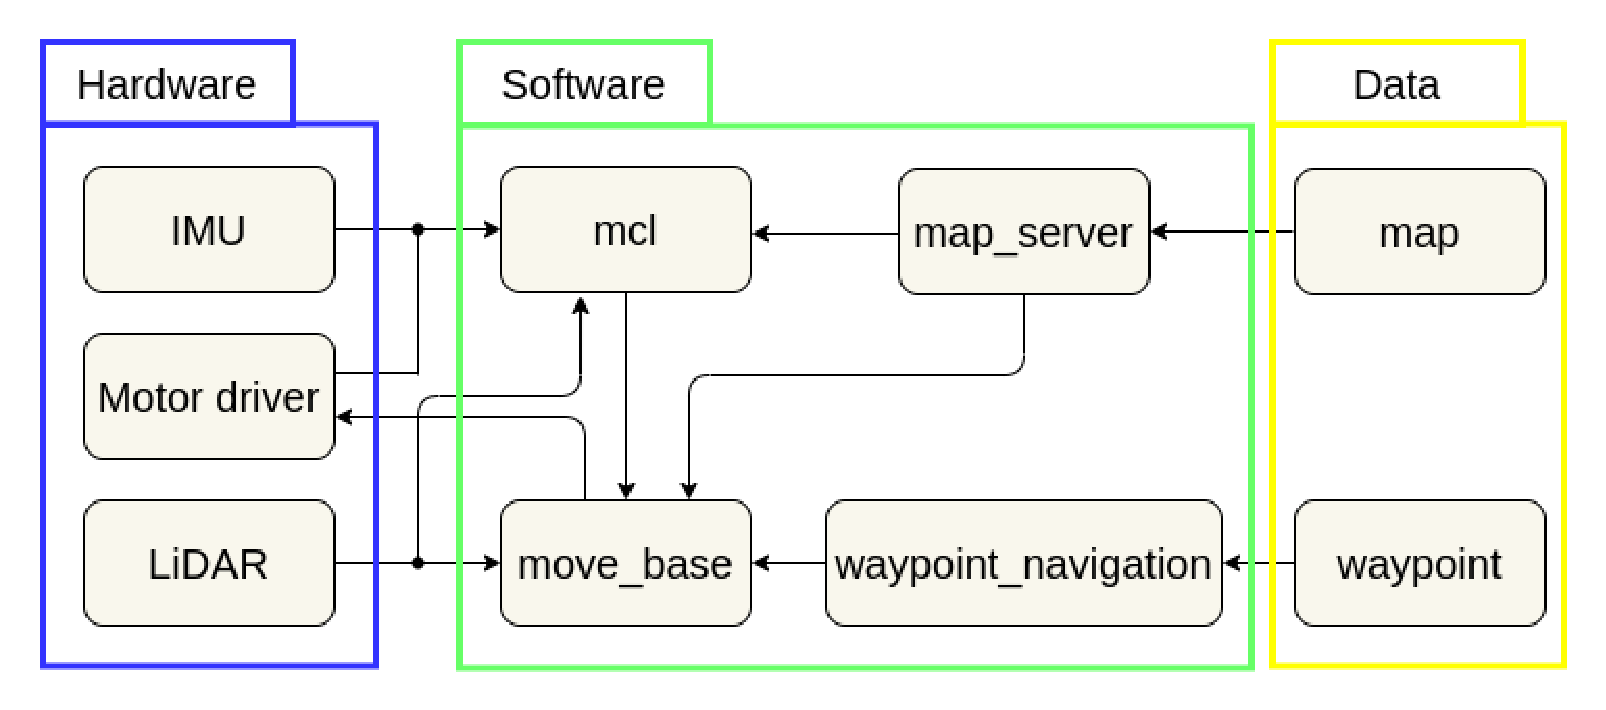
\includegraphics[width=90mm]{fig/software.pdf}
  \caption{Structure of the system.}
  \label{fig:soft-fig}
\end{figure}

\vspace*{2mm}

\section{各ロボットごとの研究開発}
本研究室では,使用するロボットごとに研究開発の目的が異なる.つくばチャレンジ2023においては,
ORNE-box2を使用するチームとORNE-box3を使用するチームの2つに分かれて研究開発を行ってきた.
以降,それぞれのチームをbox2チーム,box3チームと呼ぶこととする.
本章では,各チームごとの取り組みを述べる.

\subsection{box2チームの取り組み}
つくばチャレンジ2022において,box2チームは記録走行で完走を達成している.しかし,本走行では道路端で
一時停止に失敗し,記録は 320[m]であった.一時停止失敗の原因としては,自己位置推定の破綻が挙げられる.
ORNE-box2では,本走行前日にロボットの制御に使用していたコンピュータである Jetson AGX Xavier が
起動しなくなるトラブルが発生したため,急遽 GIGABYTE GB-BXi7H-4500 に交換を行っていた.
これにより計算処理が間に合わなかったおそれがある.

よって本年度は,基本的には昨年度と同じシステムを用いて完走することを目的とした.
なお,制御用のコンピュータには,記録走行完走時に用いていた Jetson AGX Xavier を使用した.
本年度の取り組みを以下で紹介する.

\subsubsection{低層}障害物

\subsubsection{選択課題 D1について}
ちなみに検証段階であったため,本走行での使用には至っていない.

\subsubsection{本走行の結果}
box2チームの本年度の本走行の記録は,715[m]であった.
なお,つくばチャレンジEX@イーアスにおいて,box2チームは完走を達成している.
\subsection{box3チームの取り組み}
本年度の取り組みを以下で紹介する.

\subsubsection{本走行の結果}
ああああ



\section{結言}
本稿では,千葉工業大学未来ロボティクス学科 box2,box3チームで開発しているロボットとシステムの構成に
関して述べた.また,つくばチャレンジ2023に向けた取り組みについて紹介した.\\

\section*{謝辞}
つくばチャレンジ実行委員会の皆様およびつくば市の皆様に感謝申し上げます.また,上田研究室の皆様には
つくばチャレンジ2023の参加にあたり,ご意見やご協力をいただき感謝申し上げます.\\


% 参考文献
% \small
\footnotesize
\begin{thebibliography}{99}

\bibitem{box}
井口 颯人, 石江 義規, 樋高 聖人, 上田 隆一, 林原 靖男 : “ 屋外自律移動ロ
ボットプラットフォーム ORNE-box の開発 ”, 3H2-03 , SI2021(2021)

\bibitem{navigation}
ros-planning, navigation リポジトリ\\
\url{https://github.com/ros-planning/navigation}\\
(最終閲覧日:\today)

\bibitem{orne-navigation}
open-rdc, orne\_navigation リポジトリ\\
\url{https://github.com/open-rdc/orne_navigation}\\
(最終閲覧日:\today)

\bibitem{orne-box}
open-rdc, orne-box リポジトリ\\
\url{https://github.com/open-rdc/orne-box}\\
(最終閲覧日:\today)

\bibitem{open-rdc}
Robot Design and Control Lab, open-rdc, リポジトリ\\
\url{https://github.com/open-rdc}\\
(最終閲覧日:\today)

\end{thebibliography}
\normalsize

\end{document}
